\documentclass[twoside]{article}
\usepackage{booktabs}
\usepackage{graphicx}
\usepackage[polish]{babel}
\usepackage[T1]{fontenc}
\usepackage[utf8]{inputenc}
\usepackage[table,dvipsnames]{xcolor}
\usepackage{amsmath}
\usepackage{algorithm}
\usepackage{algpseudocode}
\usepackage{titlesec}
\usepackage{fancyhdr}
\usepackage[
    a4paper,
    inner=2.5cm,   
    outer=2.5cm,   
    top=2.5cm,     
    bottom=2.5cm,  
    footskip=1cm,  
    headheight=15pt 
]{geometry}
\usepackage{float}




\definecolor{mojkolor}{RGB}{45, 45, 100}

\pagestyle{fancy}
\fancyhf{} % Wyczyszczenie domyślnych ustawień
\fancyhead[LE]{Mnożenie Macierzy}
\fancyhead[LO]{Artur Radwański - grupa 4} % Lewa strona nagłówka
\fancyhead[R]{\thepage} % Prawa strona nagłówka
\renewcommand{\headrulewidth}{0.4pt}

\titleformat{\section}
  {\normalfont\Large\bfseries\color{mojkolor}} % Styl pisma
  {\thesection}                               % Numeracja
  {1em}                                       % Odstęp
  {}                                          % Tekst przed tytułem
  [{\color{mojkolor}\titlerule[1.5pt]}]       % KRESKA PO TYTULE (bezpieczna metoda)

% Dodatkowy odstęp pod kreską, żeby tekst nie "przyklejał" się do niej
\titlespacing*{\section}{0pt}{3.5ex plus 1ex minus .2ex}{2.3ex plus .2ex}

\begin{document}
\begin{titlepage}
\centering
\Large
\vspace*{1cm}
\begin{Huge}
 \textbf{Laboratorium Algorytmów Macierzowych - ćwiczenie 1}
\end{Huge}


\vspace{0.5cm}
ćwiczenie 1 - Mnożenie Macierzy
            
 \vspace{1.5cm}

\begin{LARGE}
\textbf{Autor:}
\end{LARGE}
Artur Radwański



\vfill
            
Kraków\\ Semestr letni 2026

            
\vspace{0.8cm}

 
\includegraphics[width=0.4\textwidth]{img/agh.png}
            
Wydział Informatyki\\
Akademia Górniczo-Hutnicza\\


\end{titlepage}


\section{Środowisko}
\begin{itemize}
  \item Procesor: AMD Ryzen 7 9800X3D
  \item Pamięć: 64GB 6000MT/s
  \item Język: C++26
  \item Kompilator: gcc version 16.2.1 20260810 (GCC)
  \item System Operacyjny: 7.2.10-arch1-1
\end{itemize}

Język c++ jest językiem kompilowalnym. Kompilator tłumaczy kod źródłowy do języka mszynowego.

\section{Algorytm Bineta}

\begin{algorithm}[H]
\caption{Rekurencyjny algorytm mnożenia macierzy (Binet / Dziel i Zwyciężaj)}
\label{alg:binet}
\begin{algorithmic}[1]
\Require Macierze $A, B$ o wymiarach $N \times N$, wyzerowana macierz wynikowa $C$
\Ensure Zaktualizowana macierz $C = C + A \times B$
\Function{BinetMultiply}{$A, B, C$}
    \If{$N \le N_{base}$}
        \State \Call{NaiveMultiply}{$A, B, C, N$} \Comment{Klasyczne 3 pętle for}
        \State \Return
    \EndIf
    \State $A_{11}, A_{12}, A_{21}, A_{22} \gets $\Call{Split}{A}
    \State $B_{11}, B_{12}, B_{21}, B_{22} \gets $\Call{Split}{B}
    \State $C_{11}, C_{12}, C_{21}, C_{22} \gets $\Call{Split}{C}
    
    \State \Call{BinetMultiply}{$A_{11}, B_{11}, C_{11}$}
    \State \Call{BinetMultiply}{$A_{12}, B_{21}, C_{11}$}
    
    \State \Call{BinetMultiply}{$A_{11}, B_{12}, C_{12}$}
    \State \Call{BinetMultiply}{$A_{12}, B_{22}, C_{12}$}
    
    \State \Call{BinetMultiply}{$A_{21}, B_{11}, C_{21}$}
    \State \Call{BinetMultiply}{$A_{22}, B_{21}, C_{21}$}
    
    \State \Call{BinetMultiply}{$A_{21}, B_{12}, C_{22}$}
    \State \Call{BinetMultiply}{$A_{22}, B_{22}, C_{22}$}
\EndFunction
\end{algorithmic}
\end{algorithm}

Algorytm został zmodyfikowany, aby mógł również obsługiwać macierze prostokątne. Macierze są dzielone zamiast na 2 bloki wzdłuż ich najdłuższego wymiaru zamiast
na 4. Dla macierzy kwadratowych 3 kroki rekurencyjne modyfikacji są równoważne 1 krokowi rekurencji oryginalnego algorytmu. Dzięki temu Algorytm nie ma
problemu z macierzami których wymiar nie jest potęgą 2.

Algorytm ten ma złożoność \(O(n^3)\). Na każdym poziomie rekurencji wykonujemy 8 mnożeń, co nie przekłada się na jakikolwiek zysk względem naiwnego podejścia
iteracyjnego.


\section{Algorytm Strassena}
Algorytm strassena wykonuje jedynie 7 mnożeń na jednym poziomie rekurencji, co poprawia jego złożoność asymptotyczną. Do $O(n^{\log_{2}7})$.

\begin{algorithm}[H]
\caption{Algorytm Strassena}
\label{alg:strassen}
\begin{algorithmic}[1]
\Require Macierze $A, B$ o wymiarach $N \times N$, wyzerowana macierz wynikowa $C$
\Ensure Zaktualizowana macierz $C = C + A \times B$
\Function{StrassenMultiply}{$A, B$}
\State $N \gets \text{Length}(A)$
    \If{$N \le N_{base}$}
        \State \Return \Call{NaiveMultiply}{$A, B$}
    \EndIf
    
    \State $A_{11}, A_{12}, A_{21}, A_{22} \gets $\Call{Split}{A}
    \State $B_{11}, B_{12}, B_{21}, B_{22} \gets $\Call{Split}{B}
    \State $C_{11}, C_{12}, C_{21}, C_{22} \gets $\Call{Split}{C}
    

      \State $M_1 \gets \text{StrassenMultiply}(A_{11} + A_{22}, B_{11} + B_{22}$) \\
      \State $M_2 \gets \text{StrassenMultiply}(A_{21} + A_{22}, B_{11}$) \\
      \State $M_3 \gets \text{StrassenMultiply}(A_{11}, B_{12} - B_{22}$) \\
      \State $M_4 \gets \text{StrassenMultiply}(A_{22}, B_{21} - B_{11}$) \\
      \State $M_5 \gets \text{StrassenMultiply}(A_{11} + A_{12}, B_{22}$) \\
      \State $M_6 \gets \text{StrassenMultiply}(A_{21} - A_{11}, B_{11} + B_{12}$) \\
      \State $M_7 \gets \text{StrassenMultiply}(A_{12} - A_{22}, B_{21} + B_{22}$)
    

    
    \State $C_{11} \gets C_{11} + M_1 + M_4 - M_5 + M_7$
    \State $C_{12} \gets C_{12} + M_3 + M_5$
    \State $C_{21} \gets C_{21} + M_2 + M_4$
    \State $C_{22} \gets C_{22} + M_1 - M_2 + M_3 + M_6$
    \State \Return C
\EndFunction
\end{algorithmic}
\end{algorithm}


\subsection{Peelieng}
Aby algorytm działał dla macierzy kwadratowych, w krokach rekurencji gdzie podmacierze mają nieparzyste wymiary zastosowano Peeling

\begin{equation*}
A = \begin{pmatrix} A' & u \\ v^T & \alpha \end{pmatrix}, \quad 
B = \begin{pmatrix} B' & w \\ z^T & \beta \end{pmatrix}
\end{equation*}

Gdzie:
\begin{itemize}
    \item $A', B'$ to główne podmacierze o wymiarach $2k \times 2k$,
    \item $u, w$ to wektory kolumnowe o rozmiarze $2k \times 1$,
    \item $v^T, z^T$ to wektory wierszowe o rozmiarze $1 \times 2k$,
    \item $\alpha, \beta$ to pojedyncze wartości skalarne ($1 \times 1$).
\end{itemize}

Wynikowa macierz $C = A \cdot B$ ma postać:
\begin{equation*}
C = \begin{pmatrix} C' & x \\ y^T & \gamma \end{pmatrix}
\end{equation*}

Poszczególne składowe obliczane są w następujący sposób:
\begin{align*}
    C' &= \text{Strassen}(A', B') + u \cdot z^T \quad &\text{(Podmacierz o parzystych wymiarach )} \\
    x &= A' \cdot w + \beta \cdot u \quad &\text{(Ostatnia kolumna )} \\
    y^T &= v^T \cdot B' + \alpha \cdot z^T \quad &\text{(Ostatni wiersz )} \\
    \gamma &= v^T \cdot w + \alpha \cdot \beta \quad &\text{(Narożny skalar)}
\end{align*}

Obliczenie dodatkowego wiersza oraz kolumny poza głównym algorytmem nie wpływa na złożoność asymptotyczną, ponieważ złożoność tej operacji to $O(n^2)$, zatem
zwiększa ona jedynie narzut stały algorytmu.

\section{Algorytm Ladermana}

\begin{algorithm}[H]
\caption{Algorytm Ladermana}
\label{alg:laderman}
\begin{algorithmic}[1]
\Require Macierze $A, B$ o wymiarach $N \times N$, wyzerowana macierz wynikowa $C$
\Ensure Zaktualizowana macierz $C = C + A \times B$
\Function{L}{$A, B$}
    \If{$N \le N_{base}$}
        \State \Return \Call{NaiveMultiply}{$A, B$}
        \State 
    \EndIf
    \State $M_1 \gets L(A_{11} + A_{12} + A_{13} - A_{21} - A_{22} - A_{32} - A_{33}, B_{22})$ 
    \State $M_2 \gets L(A_{11} - A_{21}, B_{22} - B_{12})$ 
    \State $M_3 \gets L(A_{22}, B_{12} - B_{11} + B_{21} - B_{22} - B_{23} - B_{31} + B_{33}) $  
        \State $M_4 \gets L(A_{21} - A_{11} + A_{22}, B_{11} - B_{12} + B_{22}) $ 
        \State $M_5 \gets L(A_{21} + A_{22}, B_{12} - B_{11}) $ 
        \State $M_6 \gets L(A_{11}, B_{11}) $ 
        \State $M_7 \gets L(A_{31} - A_{11} + A_{32}, B_{11} - B_{13} + B_{23}) $ 
        \State $M_8 \gets L(A_{31} - A_{11}, B_{13} - B_{23}) $ 
        \State $M_9 \gets L(A_{31} + A_{32}, B_{13} - B_{11}) $ 
        \State $M_{10} \gets L(A_{11} + A_{12} + A_{13} - A_{22} - A_{23} - A_{31} - A_{32}, B_{23}) $ 
        \State $M_{11} \gets L(A_{32}, B_{13} - B_{11} + B_{21} - B_{22} - B_{23} - B_{31} + B_{32}) $ 
        \State $M_{12} \gets L(A_{32} - A_{13} + A_{33}, B_{22} + B_{31} - B_{32}) $ 
        \State $M_{13} \gets L(A_{13} - A_{33}, B_{22} - B_{32}) $ 
        \State $M_{14} \gets L(A_{13}, B_{31}) $ 
        \State $M_{15} \gets L(A_{32} + A_{33}, B_{32} - B_{31}) $ 
        \State $M_{16} \gets L(A_{22} - A_{13} + A_{23}, B_{23} + B_{31} - B_{33}) $ 
        \State $M_{17} \gets L(A_{13} - A_{23}, B_{23} - B_{33}) $ 
        \State $M_{18} \gets L(A_{22} + A_{23}, B_{33} - B_{21}) $ 
        \State $M_{19} \gets L(A_{12}, B_{21}) $ 
        \State $M_{20} \gets L(A_{23}, B_{32}) $ 
        \State $M_{21} \gets L(A_{21}, B_{13}) $ 
        \State $M_{22} \gets L(A_{31}, B_{12}) $ 
        \State $M_{23} \gets L(A_{33}, B_{33}) $
        

    \State $C_{11} \gets C_{11} + M_6 + M_{14} + M_{19}$
    \State $C_{12} \gets C_{12} + M_1 + M_4 + M_5 + M_6 + M_{12} + M_{14} + M_{15}$
    \State $C_{13} \gets C_{13} + M_6 + M_7 + M_9 + M_{10} + M_{14} + M_{16} + M_{18}$
    \State $C_{21} \gets C_{21} + M_2 + M_3 + M_4 + M_6 + M_{14} + M_{16} + M_{17}$
    \State $C_{22} \gets C_{22} + M_2 + M_4 + M_5 + M_6 + M_{20}$
    \State $C_{23} \gets C_{23} + M_{14} + M_{16} + M_{17} + M_{18} + M_{21}$
    \State $C_{31} \gets C_{31} + M_6 + M_7 + M_8 + M_{11} + M_{12} + M_{13} + M_{14}$
    \State $C_{32} \gets C_{32} + M_{12} + M_{13} + M_{14} + M_{15} + M_{22}$
    \State $C_{33} \gets C_{33} + M_6 + M_7 + M_8 + M_9 + M_{23}$
    \State \Return C
\EndFunction
\end{algorithmic}
\end{algorithm}

Algorytm wykonuje jedynie 23 mnożenia zamiast 27 co przekłada się na złożoność asymptotyczną $(n^{\log_{3}23})$. Jest to wynik nieco gorszy niż dla algorytmu
Strassena, w dodatku algorytm Ladermana alokuje znacznie więcej macierzy pomocniczych oraz wykonuje o wiele więcej dodawań, co przekłada się na gigantyczny
narzut stały.

\subsection{Peelieng}

Algorytm Ladermana wykorzystuje podział $3 \times 3$. Jeśli wymiar $N$ nie jest podzielny przez 3, reszta z dzielenia wynosi $r = N \bmod 3 \in \{1, 2\}$.
Macierze rozbijane są na główną podmacierz $3k \times 3k$ oraz brzegowe paski o szerokości $r$:

\begin{equation}
A = \begin{pmatrix} A' & U \\ V^T & \alpha \end{pmatrix}, \quad 
B = \begin{pmatrix} B' & W \\ Z^T & \beta \end{pmatrix}
\end{equation}

Gdzie:
\begin{itemize}
    \item $A', B'$ to podmacierze o wymiarach $3k \times 3k$,
    \item $U, W$ to paski pionowe o wymiarze $3k \times r$,
    \item $V^T, Z^T$ to paski poziome o wymiarze $r \times 3k$,
    \item $\alpha, \beta$ to bloki narożne o rozmiarze $r \times r$.
\end{itemize}

Rozwiązanie dla macierzy wynikowej $C = \begin{pmatrix} C' & X \\ Y^T & \Gamma \end{pmatrix}$ wylicza się analogicznie do metody Strassena, uwzględniając szersze wymiary pasków:

\begin{align}
    C' &= \text{Laderman}(A', B') + U \cdot Z^T \quad &\text{(Rdzeń } 3k \times 3k \text{ + iloczyn macierzy paskowych)} \\
    X &= A' \cdot W + U \cdot \beta \quad &\text{(Prawy pas } 3k \times r \text{)} \\
    Y^T &= V^T \cdot B' + \alpha \cdot Z^T \quad &\text{(Dolny pas } r \times 3k \text{)} \\
    \Gamma &= V^T \cdot W + \alpha \cdot \beta \quad &\text{(Narożnik } r \times r \text{)}
\end{align}

Ponieważ $r < 3$ to operacje przemnożenia pasków zachowują złożoność $O(n^2)$ ze względu na n, peeling nie zmienia więc złożoności obliczeniowej
również dla ladermana.

\section{Pomiary}
Testy wykonywano dla kwadratowych macierzy o wymiarach $n\times n$ gdzie $n \in [10, 1000]$
W komórkach macierzy zapisaono losową wartość $x \in (10^{-8}, 1)$. X były zmiennymi typu Binary64;

\subsection{Czas}
Aby zmierzyć czas wykonania algorytmu uruchamiano mnożenie 10 razy dla tej samej macierzy, po czym zapisywano uśredniony czas wykonania w milisekundach
\begin{figure}[H]
  \centering
  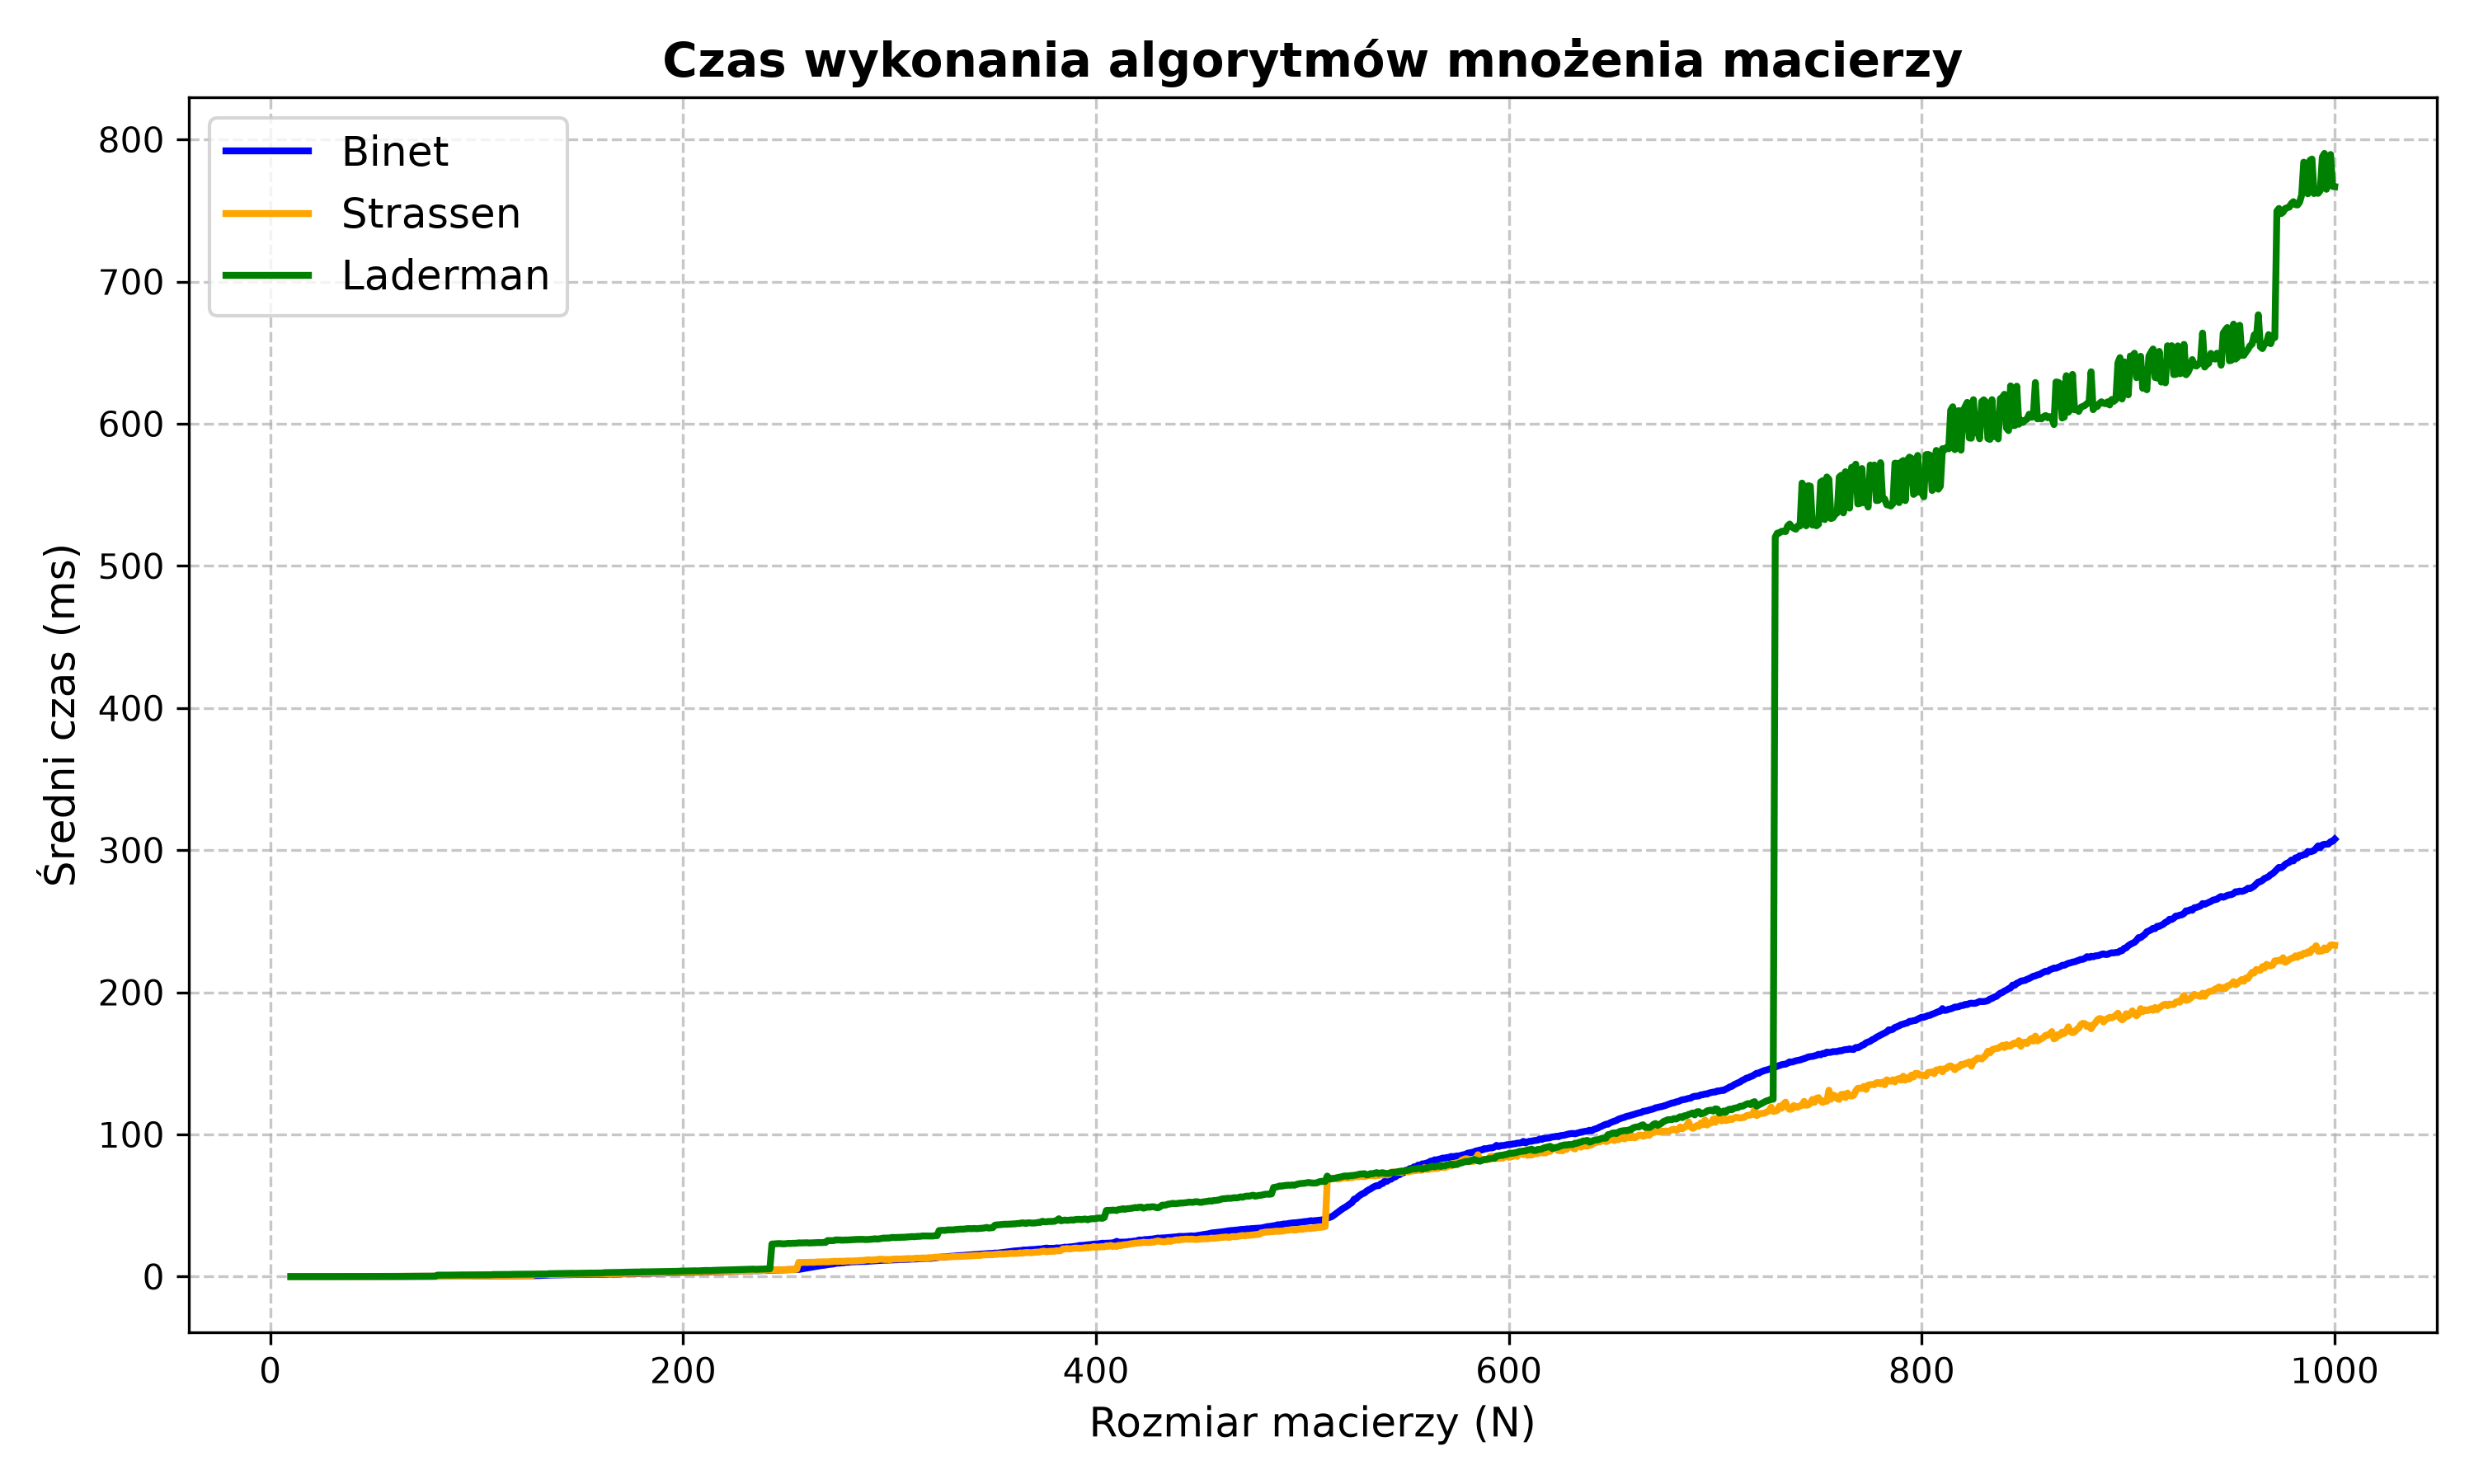
\includegraphics[width=0.9\textwidth]{img/wykres_czas.png}
  \caption{Wykres czasu wykonania algorytmów}
  \label{fig:time}
\end{figure}

Jak widać na rysunku \ref{fig:time} dla mniejszych macierzy $(n \ensuremath{<} 729)$ wszystkie algorytmy radziły sobie podobnie. Później jednak algorytm ladermana
musi wykonać dodatkowy krok rekurencji, co sprawia, że daje o wiele gorsze wyniki niż pozostałe algorytmy. Narzut z peelingu w przypadku Ladermana jest większy
niż dla Strassena, przez co widać gwałtowne skoki na wykresie, dla liczb które nie dzielą się wielokrotnie przez 3. Algorytm Strassena  zgodnie z przewidywaniami
radzi sobie najlepiej.


\subsection{FLOPS}
Liczba flops została zliczona w trakcie jednego wykonania algorytmu dla danego rozmiaru macierzy.

\begin{figure}[H]
  \centering
  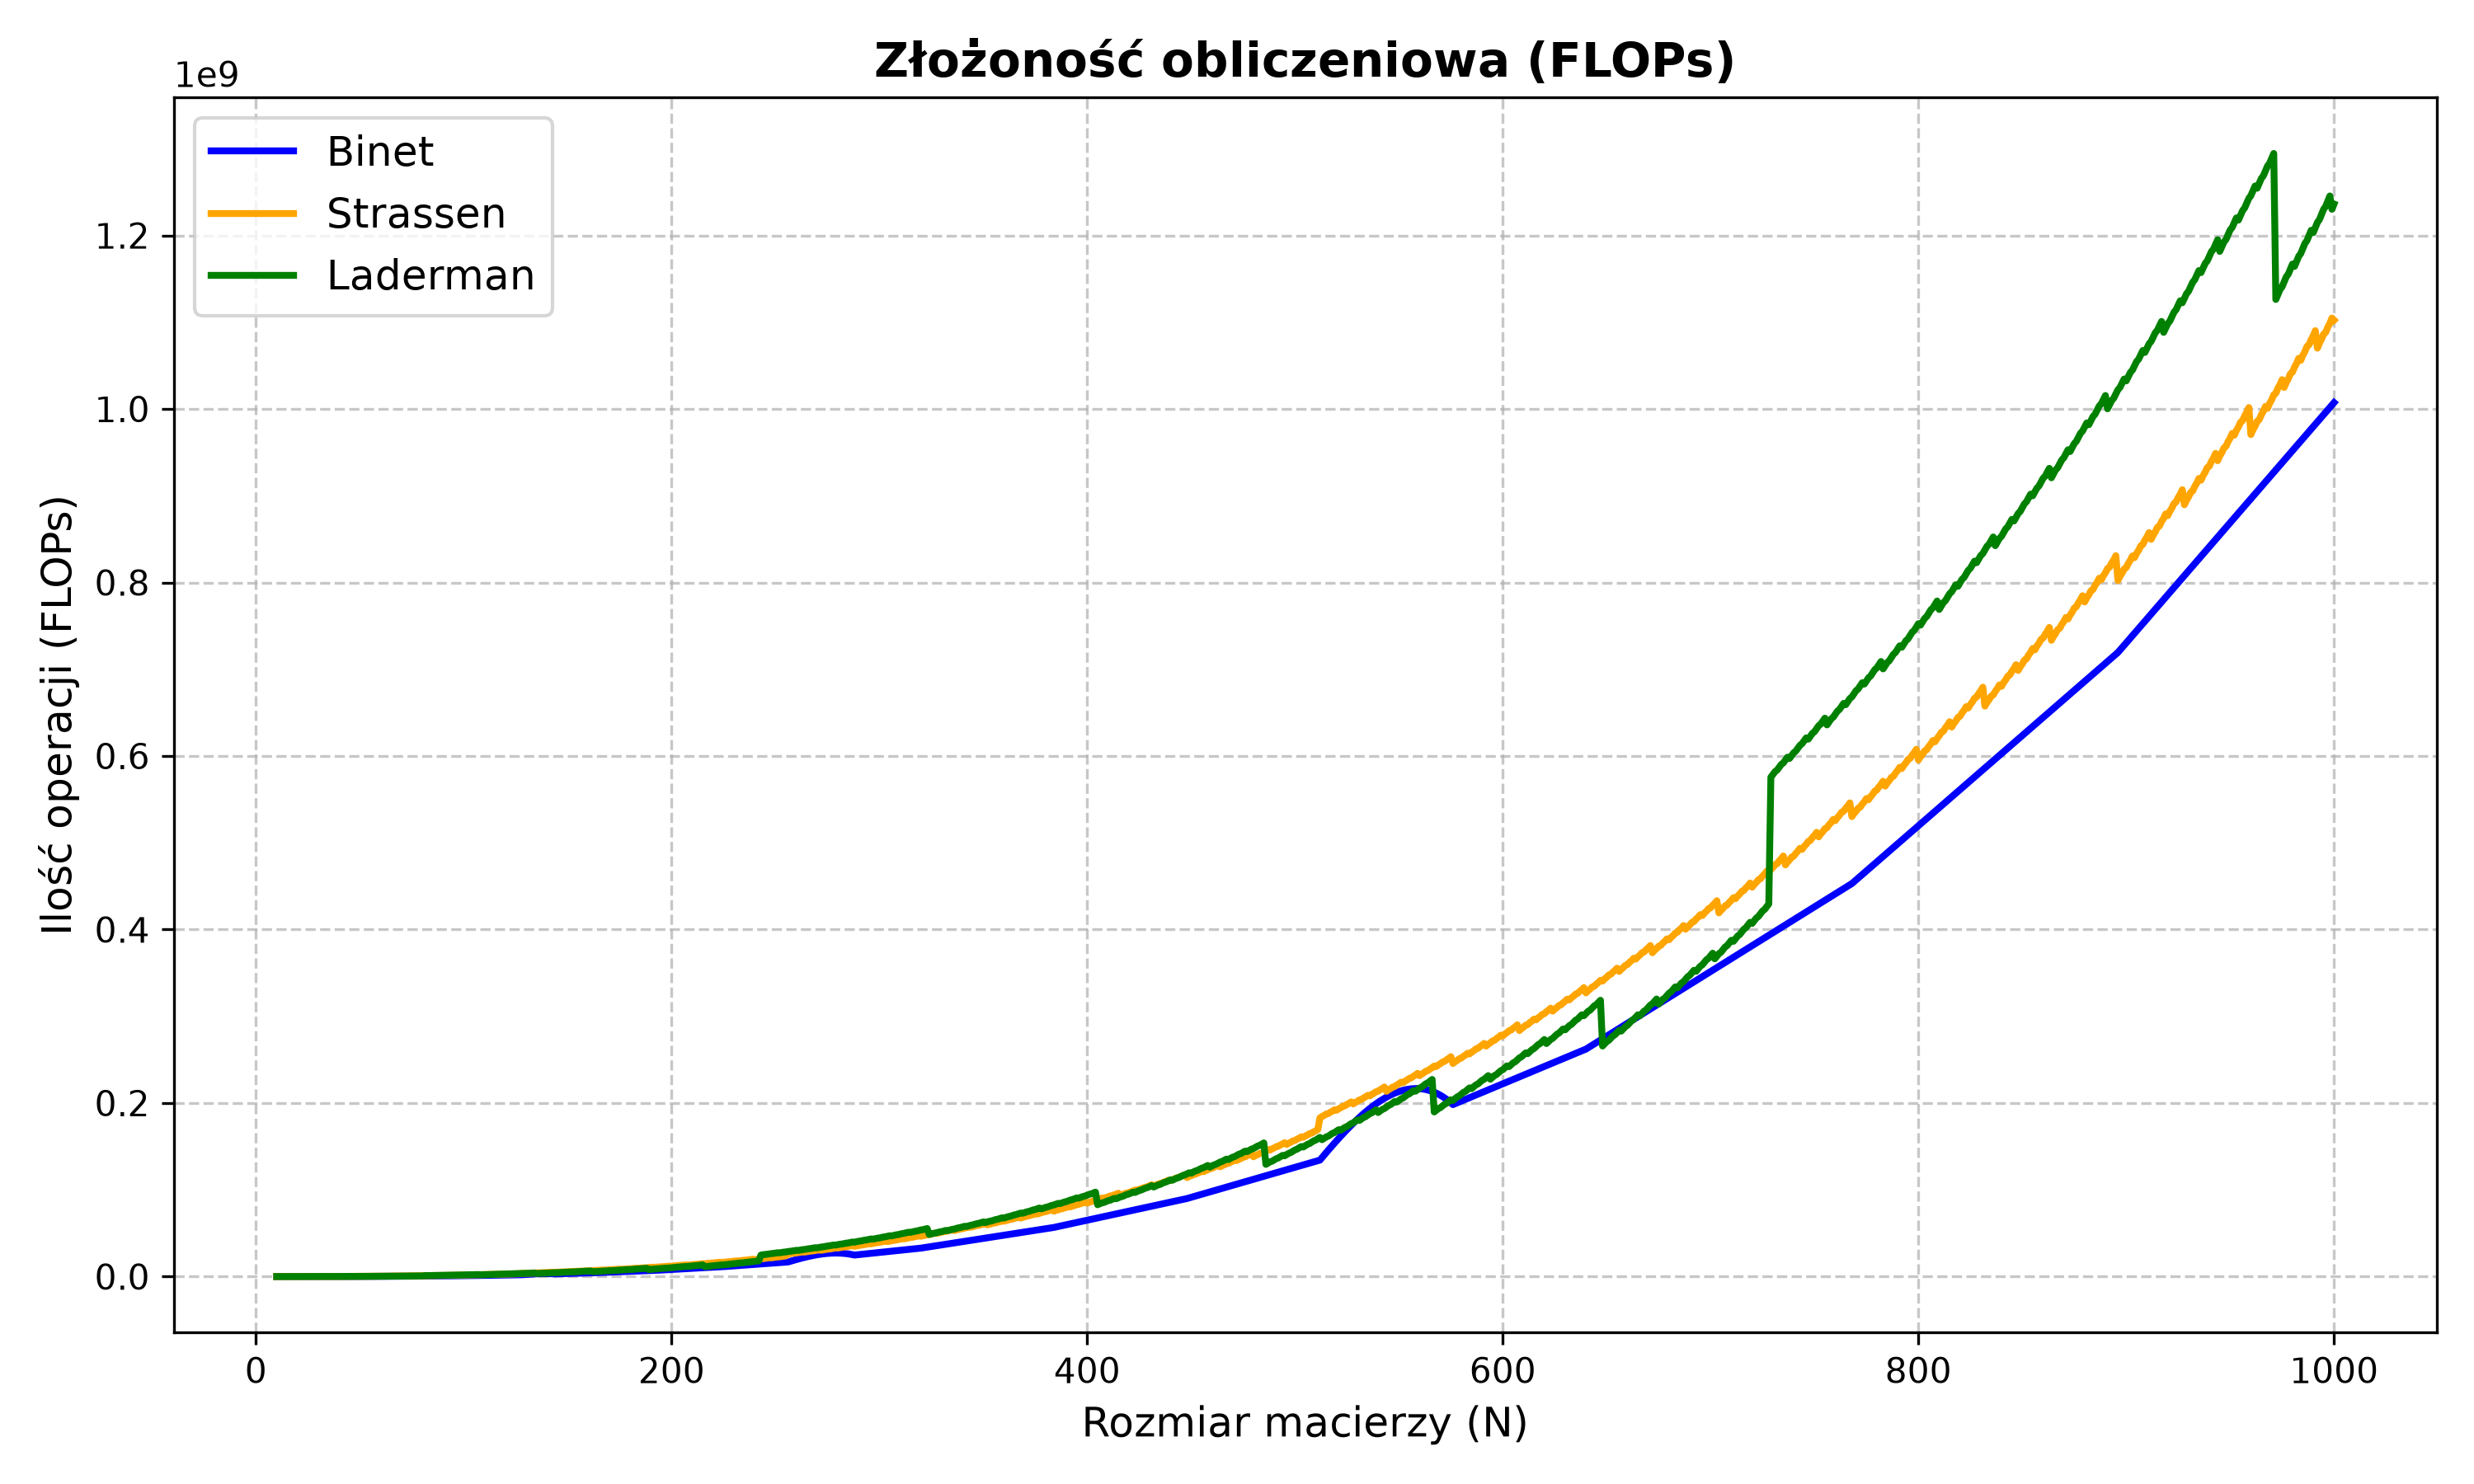
\includegraphics[width=0.9\textwidth]{img/wykres_flops.png}
  \caption{Wykres flops wykonanych w trakcie algorytmów}
  \label{fig:flops}
\end{figure}

Na rysunku widać, że dla $n = 972$ równocześnie mocno spadła liczba flops i wzrósł czas wykonania. Jest to wskazówka, że ten spadek wydajności jest 
prawdopodobnie raczej powiązany z zarządzaniem pamięcią i ładowaniem danych do L2 i L1 cache procesora niż z uwarunkowaniami artmetycznymi algorytmu.
Flops pozostałych dwóch algorytmów zachowują się w sposób przewidywalny. Pokazują one też, że zamiana dodawań na mnożenia faktycznie przynosi zyski.
Algorytm Strassena, mimo że  miał więcej flopsów, to był szybszy niż binet.

\subsection{Kontrola błędów}
Wyniki algorytmów porównano z wynikami profesjonalnej bibiloteki Eigen3 do operacji macierzowych, poniżej podano błąd maksymalny dla każdego algorytmu:
\[n = 4 \]
\begin{itemize}
  \item binet: 0
  \item strassen: 3.330669e-16
  \item laderman 2.220446e-16
\end{itemize}

\[n = 100 \]
\begin{itemize}
  \item binet: 0
  \item Strassen: 7.425172e-13
  \item Laderman: 4.263256e-14
\end{itemize}

Jak widać wszystkie wyniki mieszczą się w zakresie błędu zmiennoprzecinkowego co potwierdza ich poprawność

\end{document}